% Generated by Sphinx.
\def\sphinxdocclass{report}
\documentclass[letterpaper,10pt,english]{sphinxmanual}
\usepackage[utf8]{inputenc}
\DeclareUnicodeCharacter{00A0}{\nobreakspace}
\usepackage{cmap}
\usepackage[T1]{fontenc}
\usepackage{babel}
\usepackage{times}
\usepackage[Bjarne]{fncychap}
\usepackage{longtable}
\usepackage{sphinx}
\usepackage{multirow}


\title{AMFM\_decompy Documentation}
\date{September 20, 2014}
\release{1}
\author{Bernardo J.B. Schmitt}
\newcommand{\sphinxlogo}{}
\renewcommand{\releasename}{Release}
\makeindex

\makeatletter
\def\PYG@reset{\let\PYG@it=\relax \let\PYG@bf=\relax%
    \let\PYG@ul=\relax \let\PYG@tc=\relax%
    \let\PYG@bc=\relax \let\PYG@ff=\relax}
\def\PYG@tok#1{\csname PYG@tok@#1\endcsname}
\def\PYG@toks#1+{\ifx\relax#1\empty\else%
    \PYG@tok{#1}\expandafter\PYG@toks\fi}
\def\PYG@do#1{\PYG@bc{\PYG@tc{\PYG@ul{%
    \PYG@it{\PYG@bf{\PYG@ff{#1}}}}}}}
\def\PYG#1#2{\PYG@reset\PYG@toks#1+\relax+\PYG@do{#2}}

\expandafter\def\csname PYG@tok@gd\endcsname{\def\PYG@tc##1{\textcolor[rgb]{0.63,0.00,0.00}{##1}}}
\expandafter\def\csname PYG@tok@gu\endcsname{\let\PYG@bf=\textbf\def\PYG@tc##1{\textcolor[rgb]{0.50,0.00,0.50}{##1}}}
\expandafter\def\csname PYG@tok@gt\endcsname{\def\PYG@tc##1{\textcolor[rgb]{0.00,0.27,0.87}{##1}}}
\expandafter\def\csname PYG@tok@gs\endcsname{\let\PYG@bf=\textbf}
\expandafter\def\csname PYG@tok@gr\endcsname{\def\PYG@tc##1{\textcolor[rgb]{1.00,0.00,0.00}{##1}}}
\expandafter\def\csname PYG@tok@cm\endcsname{\let\PYG@it=\textit\def\PYG@tc##1{\textcolor[rgb]{0.25,0.50,0.56}{##1}}}
\expandafter\def\csname PYG@tok@vg\endcsname{\def\PYG@tc##1{\textcolor[rgb]{0.73,0.38,0.84}{##1}}}
\expandafter\def\csname PYG@tok@m\endcsname{\def\PYG@tc##1{\textcolor[rgb]{0.13,0.50,0.31}{##1}}}
\expandafter\def\csname PYG@tok@mh\endcsname{\def\PYG@tc##1{\textcolor[rgb]{0.13,0.50,0.31}{##1}}}
\expandafter\def\csname PYG@tok@cs\endcsname{\def\PYG@tc##1{\textcolor[rgb]{0.25,0.50,0.56}{##1}}\def\PYG@bc##1{\setlength{\fboxsep}{0pt}\colorbox[rgb]{1.00,0.94,0.94}{\strut ##1}}}
\expandafter\def\csname PYG@tok@ge\endcsname{\let\PYG@it=\textit}
\expandafter\def\csname PYG@tok@vc\endcsname{\def\PYG@tc##1{\textcolor[rgb]{0.73,0.38,0.84}{##1}}}
\expandafter\def\csname PYG@tok@il\endcsname{\def\PYG@tc##1{\textcolor[rgb]{0.13,0.50,0.31}{##1}}}
\expandafter\def\csname PYG@tok@go\endcsname{\def\PYG@tc##1{\textcolor[rgb]{0.20,0.20,0.20}{##1}}}
\expandafter\def\csname PYG@tok@cp\endcsname{\def\PYG@tc##1{\textcolor[rgb]{0.00,0.44,0.13}{##1}}}
\expandafter\def\csname PYG@tok@gi\endcsname{\def\PYG@tc##1{\textcolor[rgb]{0.00,0.63,0.00}{##1}}}
\expandafter\def\csname PYG@tok@gh\endcsname{\let\PYG@bf=\textbf\def\PYG@tc##1{\textcolor[rgb]{0.00,0.00,0.50}{##1}}}
\expandafter\def\csname PYG@tok@ni\endcsname{\let\PYG@bf=\textbf\def\PYG@tc##1{\textcolor[rgb]{0.84,0.33,0.22}{##1}}}
\expandafter\def\csname PYG@tok@nl\endcsname{\let\PYG@bf=\textbf\def\PYG@tc##1{\textcolor[rgb]{0.00,0.13,0.44}{##1}}}
\expandafter\def\csname PYG@tok@nn\endcsname{\let\PYG@bf=\textbf\def\PYG@tc##1{\textcolor[rgb]{0.05,0.52,0.71}{##1}}}
\expandafter\def\csname PYG@tok@no\endcsname{\def\PYG@tc##1{\textcolor[rgb]{0.38,0.68,0.84}{##1}}}
\expandafter\def\csname PYG@tok@na\endcsname{\def\PYG@tc##1{\textcolor[rgb]{0.25,0.44,0.63}{##1}}}
\expandafter\def\csname PYG@tok@nb\endcsname{\def\PYG@tc##1{\textcolor[rgb]{0.00,0.44,0.13}{##1}}}
\expandafter\def\csname PYG@tok@nc\endcsname{\let\PYG@bf=\textbf\def\PYG@tc##1{\textcolor[rgb]{0.05,0.52,0.71}{##1}}}
\expandafter\def\csname PYG@tok@nd\endcsname{\let\PYG@bf=\textbf\def\PYG@tc##1{\textcolor[rgb]{0.33,0.33,0.33}{##1}}}
\expandafter\def\csname PYG@tok@ne\endcsname{\def\PYG@tc##1{\textcolor[rgb]{0.00,0.44,0.13}{##1}}}
\expandafter\def\csname PYG@tok@nf\endcsname{\def\PYG@tc##1{\textcolor[rgb]{0.02,0.16,0.49}{##1}}}
\expandafter\def\csname PYG@tok@si\endcsname{\let\PYG@it=\textit\def\PYG@tc##1{\textcolor[rgb]{0.44,0.63,0.82}{##1}}}
\expandafter\def\csname PYG@tok@s2\endcsname{\def\PYG@tc##1{\textcolor[rgb]{0.25,0.44,0.63}{##1}}}
\expandafter\def\csname PYG@tok@vi\endcsname{\def\PYG@tc##1{\textcolor[rgb]{0.73,0.38,0.84}{##1}}}
\expandafter\def\csname PYG@tok@nt\endcsname{\let\PYG@bf=\textbf\def\PYG@tc##1{\textcolor[rgb]{0.02,0.16,0.45}{##1}}}
\expandafter\def\csname PYG@tok@nv\endcsname{\def\PYG@tc##1{\textcolor[rgb]{0.73,0.38,0.84}{##1}}}
\expandafter\def\csname PYG@tok@s1\endcsname{\def\PYG@tc##1{\textcolor[rgb]{0.25,0.44,0.63}{##1}}}
\expandafter\def\csname PYG@tok@gp\endcsname{\let\PYG@bf=\textbf\def\PYG@tc##1{\textcolor[rgb]{0.78,0.36,0.04}{##1}}}
\expandafter\def\csname PYG@tok@sh\endcsname{\def\PYG@tc##1{\textcolor[rgb]{0.25,0.44,0.63}{##1}}}
\expandafter\def\csname PYG@tok@ow\endcsname{\let\PYG@bf=\textbf\def\PYG@tc##1{\textcolor[rgb]{0.00,0.44,0.13}{##1}}}
\expandafter\def\csname PYG@tok@sx\endcsname{\def\PYG@tc##1{\textcolor[rgb]{0.78,0.36,0.04}{##1}}}
\expandafter\def\csname PYG@tok@bp\endcsname{\def\PYG@tc##1{\textcolor[rgb]{0.00,0.44,0.13}{##1}}}
\expandafter\def\csname PYG@tok@c1\endcsname{\let\PYG@it=\textit\def\PYG@tc##1{\textcolor[rgb]{0.25,0.50,0.56}{##1}}}
\expandafter\def\csname PYG@tok@kc\endcsname{\let\PYG@bf=\textbf\def\PYG@tc##1{\textcolor[rgb]{0.00,0.44,0.13}{##1}}}
\expandafter\def\csname PYG@tok@c\endcsname{\let\PYG@it=\textit\def\PYG@tc##1{\textcolor[rgb]{0.25,0.50,0.56}{##1}}}
\expandafter\def\csname PYG@tok@mf\endcsname{\def\PYG@tc##1{\textcolor[rgb]{0.13,0.50,0.31}{##1}}}
\expandafter\def\csname PYG@tok@err\endcsname{\def\PYG@bc##1{\setlength{\fboxsep}{0pt}\fcolorbox[rgb]{1.00,0.00,0.00}{1,1,1}{\strut ##1}}}
\expandafter\def\csname PYG@tok@kd\endcsname{\let\PYG@bf=\textbf\def\PYG@tc##1{\textcolor[rgb]{0.00,0.44,0.13}{##1}}}
\expandafter\def\csname PYG@tok@ss\endcsname{\def\PYG@tc##1{\textcolor[rgb]{0.32,0.47,0.09}{##1}}}
\expandafter\def\csname PYG@tok@sr\endcsname{\def\PYG@tc##1{\textcolor[rgb]{0.14,0.33,0.53}{##1}}}
\expandafter\def\csname PYG@tok@mo\endcsname{\def\PYG@tc##1{\textcolor[rgb]{0.13,0.50,0.31}{##1}}}
\expandafter\def\csname PYG@tok@mi\endcsname{\def\PYG@tc##1{\textcolor[rgb]{0.13,0.50,0.31}{##1}}}
\expandafter\def\csname PYG@tok@kn\endcsname{\let\PYG@bf=\textbf\def\PYG@tc##1{\textcolor[rgb]{0.00,0.44,0.13}{##1}}}
\expandafter\def\csname PYG@tok@o\endcsname{\def\PYG@tc##1{\textcolor[rgb]{0.40,0.40,0.40}{##1}}}
\expandafter\def\csname PYG@tok@kr\endcsname{\let\PYG@bf=\textbf\def\PYG@tc##1{\textcolor[rgb]{0.00,0.44,0.13}{##1}}}
\expandafter\def\csname PYG@tok@s\endcsname{\def\PYG@tc##1{\textcolor[rgb]{0.25,0.44,0.63}{##1}}}
\expandafter\def\csname PYG@tok@kp\endcsname{\def\PYG@tc##1{\textcolor[rgb]{0.00,0.44,0.13}{##1}}}
\expandafter\def\csname PYG@tok@w\endcsname{\def\PYG@tc##1{\textcolor[rgb]{0.73,0.73,0.73}{##1}}}
\expandafter\def\csname PYG@tok@kt\endcsname{\def\PYG@tc##1{\textcolor[rgb]{0.56,0.13,0.00}{##1}}}
\expandafter\def\csname PYG@tok@sc\endcsname{\def\PYG@tc##1{\textcolor[rgb]{0.25,0.44,0.63}{##1}}}
\expandafter\def\csname PYG@tok@sb\endcsname{\def\PYG@tc##1{\textcolor[rgb]{0.25,0.44,0.63}{##1}}}
\expandafter\def\csname PYG@tok@k\endcsname{\let\PYG@bf=\textbf\def\PYG@tc##1{\textcolor[rgb]{0.00,0.44,0.13}{##1}}}
\expandafter\def\csname PYG@tok@se\endcsname{\let\PYG@bf=\textbf\def\PYG@tc##1{\textcolor[rgb]{0.25,0.44,0.63}{##1}}}
\expandafter\def\csname PYG@tok@sd\endcsname{\let\PYG@it=\textit\def\PYG@tc##1{\textcolor[rgb]{0.25,0.44,0.63}{##1}}}

\def\PYGZbs{\char`\\}
\def\PYGZus{\char`\_}
\def\PYGZob{\char`\{}
\def\PYGZcb{\char`\}}
\def\PYGZca{\char`\^}
\def\PYGZam{\char`\&}
\def\PYGZlt{\char`\<}
\def\PYGZgt{\char`\>}
\def\PYGZsh{\char`\#}
\def\PYGZpc{\char`\%}
\def\PYGZdl{\char`\$}
\def\PYGZhy{\char`\-}
\def\PYGZsq{\char`\'}
\def\PYGZdq{\char`\"}
\def\PYGZti{\char`\~}
% for compatibility with earlier versions
\def\PYGZat{@}
\def\PYGZlb{[}
\def\PYGZrb{]}
\makeatother

\begin{document}

\maketitle
\tableofcontents
\phantomsection\label{index::doc}


Contents:


\chapter{pYAAPT}
\label{pYAAPT:welcome-to-amfm-decompy-s-documentation}\label{pYAAPT::doc}\label{pYAAPT:pyaapt}
This a ported version for Python from the YAAPT (Yet Another Algorithm for Pitch Tracking) algorithm. The original MATLAB program was written by Hongbing Hu and Stephen A. Zahorian.

The YAAPT program, designed for fundamental frequency tracking, is extremely robust for both high quality and telephone speech. The YAAPT program was created by the Speech Communication Laboratory of the state university of New York at Binghamton. The original program is available at \href{http://www.ws.binghamton.edu/zahorian}{http://www.ws.binghamton.edu/zahorian} as free software. Further information about the program could be found at {\hyperref[pYAAPT:ref1]{{[}ref1{]}}}.

It must be noticed that, although this ported version is almost equal to the original, some few changes were made in order to make the program more ``pythonic'' and improve its performance. Nevertheless, the results obtained with both algorithms were similar.


\section{Quick start}
\label{pYAAPT:quick-start}
The pYAAPT basically contains the whole set of functions to extract the pitch track from a speech signal. These functions, in their turn, are independent from the pyQHM package. Therefore, pYAAPT can be used in any other speech processing application, not only in the AM-FM decomposition.

USAGE:
\index{yaapt() (in module amfm\_decompy.pYAAPT)}

\begin{fulllineitems}
\phantomsection\label{pYAAPT:amfm_decompy.pYAAPT.yaapt}\pysiglinewithargsret{\code{amfm\_decompy.pYAAPT.}\bfcode{yaapt}}{\emph{signal}\optional{, \emph{options}}}{}~\begin{quote}\begin{description}
\item[{Parameters}] \leavevmode\begin{itemize}
\item {} 
\textbf{signal} (\emph{signal object}) -- created with amfm\_decompy.basic\_tools.

\item {} 
\textbf{options} (Must be formatted as follow: {\color{red}\bfseries{}**}\{`option\_name1' : value1,   `option\_name2' : value2, ...\}) -- the default configuration values for all of them are the same as in the original version. A short description about them is presented in the next subitem. For more information about them, please refer to {\hyperref[pYAAPT:ref1]{{[}ref1{]}}}.

\end{itemize}

\item[{Return type}] \leavevmode
pitch object

\end{description}\end{quote}

\end{fulllineitems}


OPTIONS:
\begin{itemize}
\item {} 
`frame\_length' - length of each analysis frame (default: 25 ms)

\item {} 
`frame\_space' - spacing between analysis frames (default: 10 ms)

\item {} 
`f0\_min' - minimum pitch searched (default: 60 Hz)

\item {} 
`f0\_max' - maximum pitch searched (default: 400 Hz)

\item {} 
`fft\_length' - FFT length (default: 8192 samples)

\item {} 
`bp\_forder' - order of band-pass filter (default: 150)

\item {} 
`bp\_low' - low frequency of filter passband (default: 50 Hz)

\item {} 
`bp\_high' - high frequency of filter passband (default: 1500 Hz)

\item {} 
`nlfer\_thresh1' - NLFER (Normalized Low Frequency Energy Ratio) boundary for voiced/unvoiced decisions (default: 0.75)

\item {} 
`nlfer\_thresh2' - threshold for NLFER definitely unvoiced (default: 0.1)

\item {} 
`shc\_numharms' - number of harmonics in SHC (Spectral Harmonics Correlation) calculation (default: 3)

\item {} 
`shc\_window' - SHC window length (default: 40 Hz)

\item {} 
`shc\_maxpeaks' - maximum number of SHC peaks to be found (default: 4)

\item {} 
`shc\_pwidth' - window width in SHC peak picking (default: 50 Hz)

\item {} 
`shc\_thresh1' - threshold 1 for SHC peak picking (default: 5)

\item {} 
`shc\_thresh2' - threshold 2 for SHC peak picking (default: 1.25)

\item {} 
`f0\_double'- pitch doubling decision threshold (default: 150 Hz)

\item {} 
`f0\_half' - pitch halving decision threshold (default: 150 Hz)

\item {} 
`dp5\_k1' - weight used in dynamic program (default: 11)

\item {} 
`dec\_factor' - factor for signal resampling (default: 1)

\item {} 
`nccf\_thresh1' - threshold for considering a peak in NCCF (Normalized Cross Correlation Function) (default: 0.25)

\item {} 
`nccf\_thresh2' - threshold for terminating search in NCCF (default: 0.9)

\item {} 
`nccf\_maxcands' - maximum number of candidates found (default: 3)

\item {} 
`nccf\_pwidth' - window width in NCCF peak picking (default: 5)

\item {} 
`merit\_boost' - boost merit (default. 0.20)

\item {} 
`merit\_pivot' - merit assigned to unvoiced candidates in definitely unvoiced frames (default: 0.99)

\item {} 
`merit\_extra' - merit assigned to extra candidates in reducing pitch doubling/halving errors (default: 0.4)

\item {} 
`median\_value' - order of medial filter (default: 7)

\item {} 
`dp\_w1' - DP (Dynamic Programming) weight factor for voiced-voiced transitions (default: 0.15)

\item {} 
`dp\_w2' - DP weight factor for voiced-unvoiced or unvoiced-voiced transitions (default: 0.5)

\item {} 
`dp\_w3' - DP weight factor of unvoiced-unvoiced transitions (default: 0.1)

\item {} 
`dp\_w4' - Weight factor for local costs (default: 0.9)

\end{itemize}

EXAMPLES:

Example 1 - extract the pitch track from a signal using the default configurations:

\begin{Verbatim}[commandchars=\\\{\}]
\PYG{k+kn}{import} \PYG{n+nn}{amfm\PYGZus{}decompy.pYAAPT} \PYG{k+kn}{as} \PYG{n+nn}{pYAAPT}
\PYG{k+kn}{import} \PYG{n+nn}{amfm\PYGZus{}decompy.basic\PYGZus{}tools} \PYG{k+kn}{as} \PYG{n+nn}{basic}

\PYG{n}{signal} \PYG{o}{=} \PYG{n}{basic}\PYG{o}{.}\PYG{n}{SignalObj}\PYG{p}{(}\PYG{l+s}{\PYGZsq{}}\PYG{l+s}{path\PYGZus{}to\PYGZus{}sample.wav}\PYG{l+s}{\PYGZsq{}}\PYG{p}{)}
\PYG{n}{pitch} \PYG{o}{=} \PYG{n}{pYAAPT}\PYG{o}{.}\PYG{n}{yaapt}\PYG{p}{(}\PYG{n}{signal}\PYG{p}{)}
\end{Verbatim}

Example 2 - extract the pitch track from a signal with the minimum pitch set to 150 Hz, the frame length to 15 ms and the frame jump to 5 ms:

\begin{Verbatim}[commandchars=\\\{\}]
\PYG{k+kn}{import} \PYG{n+nn}{amfm\PYGZus{}decompy.pYAAPT} \PYG{k+kn}{as} \PYG{n+nn}{pYAAPT}
\PYG{k+kn}{import} \PYG{n+nn}{amfm\PYGZus{}decompy.basic\PYGZus{}tools} \PYG{k+kn}{as} \PYG{n+nn}{basic}

\PYG{n}{signal} \PYG{o}{=} \PYG{n}{basic}\PYG{o}{.}\PYG{n}{SignalObj}\PYG{p}{(}\PYG{l+s}{\PYGZsq{}}\PYG{l+s}{path\PYGZus{}to\PYGZus{}sample.wav}\PYG{l+s}{\PYGZsq{}}\PYG{p}{)}
\PYG{n}{pitch} \PYG{o}{=} \PYG{n}{pYAAPT}\PYG{o}{.}\PYG{n}{yaapt}\PYG{p}{(}\PYG{n}{signal}\PYG{p}{,} \PYG{o}{*}\PYG{o}{*}\PYG{p}{\PYGZob{}}\PYG{l+s}{\PYGZsq{}}\PYG{l+s}{f0\PYGZus{}min}\PYG{l+s}{\PYGZsq{}} \PYG{p}{:} \PYG{l+m+mf}{150.0}\PYG{p}{,} \PYG{l+s}{\PYGZsq{}}\PYG{l+s}{frame\PYGZus{}length}\PYG{l+s}{\PYGZsq{}} \PYG{p}{:} \PYG{l+m+mf}{15.0}\PYG{p}{,} \PYG{l+s}{\PYGZsq{}}\PYG{l+s}{frame\PYGZus{}space}\PYG{l+s}{\PYGZsq{}} \PYG{p}{:} \PYG{l+m+mf}{5.0}\PYG{p}{\PYGZcb{}}\PYG{p}{)}
\end{Verbatim}


\section{Classes}
\label{pYAAPT:classes}

\subsection{PitchObj Class}
\label{pYAAPT:pitchobj-class}
The PitchObj Class stores the extracted pitch and all the parameters related to it. A pitch object is necessary for the QHM algorithms. However, the pitch class structure was built in a way that it can be used by any other pitch tracker, not only the YAAPT.

USAGE:
\index{PitchObj() (in module amfm\_decompy.pYAAPT)}

\begin{fulllineitems}
\phantomsection\label{pYAAPT:amfm_decompy.pYAAPT.PitchObj}\pysiglinewithargsret{\code{amfm\_decompy.pYAAPT.}\bfcode{PitchObj}}{\emph{frame\_size}, \emph{frame\_jump}\optional{, \emph{nfft=8192}}}{}~\begin{quote}\begin{description}
\item[{Parameters}] \leavevmode\begin{itemize}
\item {} 
\textbf{frame\_size} (\emph{int}) -- analysis frame length.

\item {} 
\textbf{frame\_jump} (\emph{int}) -- distance between the center of a extracting frame and the center of its adjacent neighbours.

\item {} 
\textbf{nfft} (\emph{int}) -- FFT length.

\end{itemize}

\item[{Return type}] \leavevmode
pitch object.

\end{description}\end{quote}

\end{fulllineitems}



\subsubsection{PITCH CLASS VARIABLES:}
\label{pYAAPT:pitch-class-variables}
These variables not related with the YAAPT algorithm itself, but with a post-processing where the data is smoothed and halving/doubling errors corrected.
\index{PITCH\_HALF (in module PitchObj)}

\begin{fulllineitems}
\phantomsection\label{pYAAPT:PitchObj.PITCH_HALF}\pysigline{\code{PitchObj.}\bfcode{PITCH\_HALF}}
This variable is a flag. When its value is equal to 1, the halving detector set the half pitch values to 0. If PITCH\_HALF is equal to 2, the half pitch values are multiplied by 2. For other PITCH\_HALF values, the halving detector is not employed (default: 0).

\end{fulllineitems}

\index{PITCH\_HALF\_SENS (in module PitchObj)}

\begin{fulllineitems}
\phantomsection\label{pYAAPT:PitchObj.PITCH_HALF_SENS}\pysigline{\code{PitchObj.}\bfcode{PITCH\_HALF\_SENS}}
Set the halving detector sensibility. A pitch sample is considered half valued if it is not zero and lower than:

mean(pitch) - PITCH\_HALF\_SENS*std(pitch)

(default: 2.9).

\end{fulllineitems}

\index{PITCH\_DOUBLE (in module PitchObj)}

\begin{fulllineitems}
\phantomsection\label{pYAAPT:PitchObj.PITCH_DOUBLE}\pysigline{\code{PitchObj.}\bfcode{PITCH\_DOUBLE}}
This variable is a flag. When its value is equal to 1, the doubling detector set the double pitch values to 0. If PITCH\_DOUBLE is equal to 2, the double pitch values are divided by 2. For other PITCH\_DOUBLE values, the doubling detector is not employed (default: 0).

\end{fulllineitems}

\index{PITCH\_DOUBLE\_SENS (in module PitchObj)}

\begin{fulllineitems}
\phantomsection\label{pYAAPT:PitchObj.PITCH_DOUBLE_SENS}\pysigline{\code{PitchObj.}\bfcode{PITCH\_DOUBLE\_SENS}}
Set the doubling detector sensibility. A pitch sample is considered double valued if it is not zero and higher than:

mean(pitch) + PITCH\_DOUBLE\_SENS*std(pitch)

(default: 2.9).

\end{fulllineitems}

\index{SMOOTH\_FACTOR (in module PitchObj)}

\begin{fulllineitems}
\phantomsection\label{pYAAPT:PitchObj.SMOOTH_FACTOR}\pysigline{\code{PitchObj.}\bfcode{SMOOTH\_FACTOR}}
Determines the median filter length used to smooth the interpolated pitch values (default: 5). \footnote{
don't mistake this interpolation with the one performed by the pYAAPT.upsample method. For more explanation, please refer to the pYAAPT.samp\_interp and pYAAPT.values\_interp attributes.
}

\end{fulllineitems}

\index{SMOOTH (in module PitchObj)}

\begin{fulllineitems}
\phantomsection\label{pYAAPT:PitchObj.SMOOTH}\pysigline{\code{PitchObj.}\bfcode{SMOOTH}}
This variable is a flag. When its value is not equal to 0, the interpolated pitch is smoothed by a median filter (default: 5). \footnotemark[1]

\end{fulllineitems}

\index{PTCH\_TYP (in module PitchObj)}

\begin{fulllineitems}
\phantomsection\label{pYAAPT:PitchObj.PTCH_TYP}\pysigline{\code{PitchObj.}\bfcode{PTCH\_TYP}}
If there are less than 2 voiced frames in the file, the PTCH\_TYP value is used in the interpolation (default: 100 Hz). \footnotemark[1]

\end{fulllineitems}


EXAMPLE:

Example 1 - the pitch is extracted from sample.wav with different smoothing and interpolation configurations:

\begin{Verbatim}[commandchars=\\\{\}]
\PYG{k+kn}{import} \PYG{n+nn}{amfm\PYGZus{}decompy.pYAAPT} \PYG{k+kn}{as} \PYG{n+nn}{pYAAPT}
\PYG{k+kn}{import} \PYG{n+nn}{amfm\PYGZus{}decompy.basic\PYGZus{}tools} \PYG{k+kn}{as} \PYG{n+nn}{basic}

\PYG{n}{signal} \PYG{o}{=} \PYG{n}{basic}\PYG{o}{.}\PYG{n}{SignalObj}\PYG{p}{(}\PYG{l+s}{\PYGZsq{}}\PYG{l+s}{path\PYGZus{}to\PYGZus{}sample.wav}\PYG{l+s}{\PYGZsq{}}\PYG{p}{)}

\PYG{n}{pYAAPT}\PYG{o}{.}\PYG{n}{PitchObj}\PYG{o}{.}\PYG{n}{PITCH\PYGZus{}DOUBLE} \PYG{o}{=} \PYG{l+m+mi}{2}      \PYG{c}{\PYGZsh{} set new values}
\PYG{n}{pYAAPT}\PYG{o}{.}\PYG{n}{PitchObj}\PYG{o}{.}\PYG{n}{PITCH\PYGZus{}HALF} \PYG{o}{=} \PYG{l+m+mi}{2}
\PYG{n}{pYAAPT}\PYG{o}{.}\PYG{n}{PitchObj}\PYG{o}{.}\PYG{n}{SMOOTH\PYGZus{}FACTOR} \PYG{o}{=} \PYG{l+m+mi}{3}

\PYG{n}{pitch} \PYG{o}{=} \PYG{n}{pYAAPT}\PYG{o}{.}\PYG{n}{yaapt}\PYG{p}{(}\PYG{n}{signal}\PYG{p}{)} \PYG{c}{\PYGZsh{} calculate the pitch track}
\end{Verbatim}


\subsubsection{PITCH OBJECT ATTRIBUTES:}
\label{pYAAPT:pitch-object-attributes}\index{nfft (in module PitchObj)}

\begin{fulllineitems}
\phantomsection\label{pYAAPT:PitchObj.nfft}\pysigline{\code{PitchObj.}\bfcode{nfft}}
Length in samples from the FFT used by the pitch tracker. It is set during the object's initialization.

\end{fulllineitems}

\index{frame\_size (in module PitchObj)}

\begin{fulllineitems}
\phantomsection\label{pYAAPT:PitchObj.frame_size}\pysigline{\code{PitchObj.}\bfcode{frame\_size}}
Length in samples from the frames used by the pitch tracker. It is set during the object's initialization.

\end{fulllineitems}

\index{frame\_jump (in module PitchObj)}

\begin{fulllineitems}
\phantomsection\label{pYAAPT:PitchObj.frame_jump}\pysigline{\code{PitchObj.}\bfcode{frame\_jump}}
Distance in samples between the center of a extracting frame and the center of its adjacent neighbours. It is set during the object's initialization.

\end{fulllineitems}

\index{noverlap (in module PitchObj)}

\begin{fulllineitems}
\phantomsection\label{pYAAPT:PitchObj.noverlap}\pysigline{\code{PitchObj.}\bfcode{noverlap}}
It's the difference between the frame size and the frame jump. Represents the number of samples that two adjacent frames share in common, i.e, how much they overlap each other. It is set during the object's initialization.

\end{fulllineitems}

\index{mean\_energy (in module PitchObj)}

\begin{fulllineitems}
\phantomsection\label{pYAAPT:PitchObj.mean_energy}\pysigline{\code{PitchObj.}\bfcode{mean\_energy}}
Signal's low frequency band mean energy. It is set by the PitchObj.set\_energy method.

\end{fulllineitems}

\index{energy (in module PitchObj)}

\begin{fulllineitems}
\phantomsection\label{pYAAPT:PitchObj.energy}\pysigline{\code{PitchObj.}\bfcode{energy}}
Array that contains the low frequency band energy from each frame, normalized by PitchObj.mean\_energy. It is set by the PitchObj.set\_energy method.

\end{fulllineitems}

\index{vuv (in module PitchObj)}

\begin{fulllineitems}
\phantomsection\label{pYAAPT:PitchObj.vuv}\pysigline{\code{PitchObj.}\bfcode{vuv}}
Boolean vector that indicates if each speech frame was classified as voiced (represented as `True') or unvoiced (represented as `False'). It is set by the PitchObj.set\_energy method.

\end{fulllineitems}

\index{frames\_pos (in module PitchObj)}

\begin{fulllineitems}
\phantomsection\label{pYAAPT:PitchObj.frames_pos}\pysigline{\code{PitchObj.}\bfcode{frames\_pos}}
A numpy array that contains the samples where the center of the frames were placed during the extraction. It is set by the PitchObj.set\_frame\_pos method.

\end{fulllineitems}

\index{nframes (in module PitchObj)}

\begin{fulllineitems}
\phantomsection\label{pYAAPT:PitchObj.nframes}\pysigline{\code{PitchObj.}\bfcode{nframes}}
Number of frames. It is set by the PitchObj.set\_frame\_pos method.

\end{fulllineitems}

\index{samp\_values (in module PitchObj)}\index{samp\_interp (in module PitchObj)}

\begin{fulllineitems}
\phantomsection\label{pYAAPT:PitchObj.samp_values}\pysigline{\code{PitchObj.}\bfcode{samp\_values}}\phantomsection\label{pYAAPT:PitchObj.samp_interp}\pysigline{\code{PitchObj.}\bfcode{samp\_interp}}
Both arrays contain the pitch values from each of the nframes. The only difference is that, in PitchObj.samp\_interp the unvoiced segments are substituted by the interpolation from the adjacent voiced segments edges. This provides a non-zero version from the pitch track, which can be necessary for some applications. The figure below presents both arrays from the sample.wav file:

\end{fulllineitems}


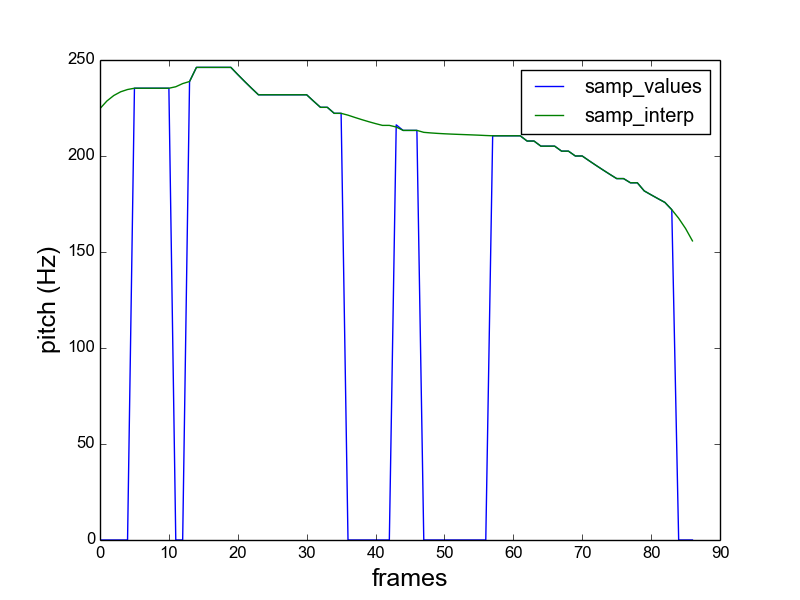
\includegraphics{samp_values.png}

Both attributes are set by the PitchObj.set\_values method.
\index{values (in module PitchObj)}\index{values\_interp (in module PitchObj)}

\begin{fulllineitems}
\phantomsection\label{pYAAPT:PitchObj.values}\pysigline{\code{PitchObj.}\bfcode{values}}\phantomsection\label{pYAAPT:PitchObj.values_interp}\pysigline{\code{PitchObj.}\bfcode{values\_interp}}
PitchObj.values and PitchObj.values\_interp are the upsampled versions from PitchObj.samp\_values and PitchObj.samp\_interp respectively. Therefore, their length is equal to the original file length (for more information, check the PitchObj.upsample() method). The figure below presents both arrays from the sample.wav file:

\end{fulllineitems}


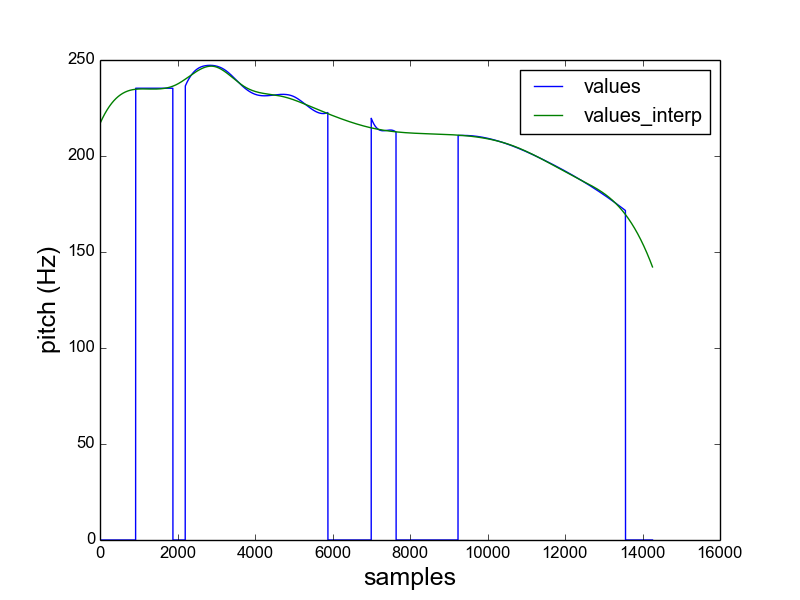
\includegraphics{values.png}

Both attributes are set by the PitchObj.set\_values method.
\index{edges (in module PitchObj)}

\begin{fulllineitems}
\phantomsection\label{pYAAPT:PitchObj.edges}\pysigline{\code{PitchObj.}\bfcode{edges}}
A list that contains the index where occur the transitions between unvoiced-voiced and voiced-unvoiced in PitchObj.values. It is set by the PitchObj.set\_values method, which employs internally the PitchObj.edges\_finder method.

\end{fulllineitems}



\subsubsection{PITCH OBJECT METHODS:}
\label{pYAAPT:pitch-object-methods}\index{set\_energy() (in module PitchObj)}

\begin{fulllineitems}
\phantomsection\label{pYAAPT:PitchObj.set_energy}\pysiglinewithargsret{\code{PitchObj.}\bfcode{set\_energy}}{\emph{energy}, \emph{threshold}}{}~\begin{quote}\begin{description}
\item[{Parameters}] \leavevmode\begin{itemize}
\item {} 
\textbf{energy} (\emph{numpy array}) -- contains the low frequency energy for each frame.

\item {} 
\textbf{threshold} -- normalized threshold.

\end{itemize}

\end{description}\end{quote}

Set the normalized low frequency energy by taking the input array and dividing it by its mean value. Normalized values above the threshold are considered voiced frames, while the ones below it are unvoiced frames.

\end{fulllineitems}

\index{set\_frames\_pos() (in module PitchObj)}

\begin{fulllineitems}
\phantomsection\label{pYAAPT:PitchObj.set_frames_pos}\pysiglinewithargsret{\code{PitchObj.}\bfcode{set\_frames\_pos}}{\emph{frames\_pos}}{}~\begin{quote}\begin{description}
\item[{Parameters}] \leavevmode
\textbf{frames\_pos} -- index with the sample positions.

\end{description}\end{quote}

Set the position from the center of the extraction frames.

\end{fulllineitems}

\index{set\_values() (in module PitchObj)}

\begin{fulllineitems}
\phantomsection\label{pYAAPT:PitchObj.set_values}\pysiglinewithargsret{\code{PitchObj.}\bfcode{set\_values}}{\emph{samp\_values}, \emph{file\_size}\optional{, \emph{interp\_tech='spline'}}}{}~\begin{quote}\begin{description}
\item[{Parameters}] \leavevmode\begin{itemize}
\item {} 
\textbf{samp\_values} (\emph{numpy array}) -- pitch value for each frame.

\item {} 
\textbf{file\_size} (\emph{int}) -- length of the speech signal.

\item {} 
\textbf{interp\_tech} (\emph{string}) -- interpolation method employed to upsample the data. Can be `spline' (default) and `step'.

\end{itemize}

\end{description}\end{quote}

Set the pitch values and also calculates its interpolated version (for more information, check the PitchObj.samp\_values and PitchObj.samp\_interp attributes). A post-process is employed then using the PitchObj class attributes. After that, both arrays are upsampled, so that the output arrays have the same length as the original speech signal. In this process, a second interpolation is necessary. The interpolation technique employed is indicated by the parameter interp\_tech.

Example:

\begin{Verbatim}[commandchars=\\\{\}]
\PYG{k+kn}{import} \PYG{n+nn}{amfm\PYGZus{}decompy.pYAAPT} \PYG{k+kn}{as} \PYG{n+nn}{pYAAPT}
\PYG{k+kn}{import} \PYG{n+nn}{amfm\PYGZus{}decompy.basic\PYGZus{}tools} \PYG{k+kn}{as} \PYG{n+nn}{basic}
\PYG{k+kn}{from} \PYG{n+nn}{matplotlib} \PYG{k+kn}{import} \PYG{n}{pyplot} \PYG{k}{as} \PYG{n}{plt}

\PYG{n}{signal} \PYG{o}{=} \PYG{n}{basic}\PYG{o}{.}\PYG{n}{SignalObj}\PYG{p}{(}\PYG{l+s}{\PYGZsq{}}\PYG{l+s}{path\PYGZus{}to\PYGZus{}sample.wav}\PYG{l+s}{\PYGZsq{}}\PYG{p}{)}
\PYG{n}{pitch} \PYG{o}{=} \PYG{n}{pYAAPT}\PYG{o}{.}\PYG{n}{yaapt}\PYG{p}{(}\PYG{n}{signal}\PYG{p}{)}

\PYG{n}{plt}\PYG{o}{.}\PYG{n}{plot}\PYG{p}{(}\PYG{n}{pitch}\PYG{o}{.}\PYG{n}{values}\PYG{p}{,} \PYG{n}{label}\PYG{o}{=}\PYG{l+s}{\PYGZsq{}}\PYG{l+s}{spline interpolation}\PYG{l+s}{\PYGZsq{}}\PYG{p}{,} \PYG{n}{color}\PYG{o}{=}\PYG{l+s}{\PYGZsq{}}\PYG{l+s}{red}\PYG{l+s}{\PYGZsq{}}\PYG{p}{)}

\PYG{n}{pitch}\PYG{o}{.}\PYG{n}{set\PYGZus{}values}\PYG{p}{(}\PYG{n}{pitch}\PYG{o}{.}\PYG{n}{samp\PYGZus{}values}\PYG{p}{,} \PYG{n+nb}{len}\PYG{p}{(}\PYG{n}{pitch}\PYG{o}{.}\PYG{n}{values}\PYG{p}{)}\PYG{p}{,} \PYG{n}{interp\PYGZus{}tech}\PYG{o}{=}\PYG{l+s}{\PYGZsq{}}\PYG{l+s}{step}\PYG{l+s}{\PYGZsq{}}\PYG{p}{)}

\PYG{n}{plt}\PYG{o}{.}\PYG{n}{plot}\PYG{p}{(}\PYG{n}{pitch}\PYG{o}{.}\PYG{n}{values}\PYG{p}{,} \PYG{n}{label}\PYG{o}{=}\PYG{l+s}{\PYGZsq{}}\PYG{l+s}{step interpolation}\PYG{l+s}{\PYGZsq{}}\PYG{p}{)}

\PYG{n}{plt}\PYG{o}{.}\PYG{n}{xlabel}\PYG{p}{(}\PYG{l+s}{\PYGZsq{}}\PYG{l+s}{samples}\PYG{l+s}{\PYGZsq{}}\PYG{p}{,} \PYG{n}{fontsize}\PYG{o}{=}\PYG{l+m+mi}{18}\PYG{p}{)}
\PYG{n}{plt}\PYG{o}{.}\PYG{n}{ylabel}\PYG{p}{(}\PYG{l+s}{\PYGZsq{}}\PYG{l+s}{pitch (Hz)}\PYG{l+s}{\PYGZsq{}}\PYG{p}{,} \PYG{n}{fontsize}\PYG{o}{=}\PYG{l+m+mi}{18}\PYG{p}{)}
\PYG{n}{plt}\PYG{o}{.}\PYG{n}{legend}\PYG{p}{(}\PYG{n}{loc}\PYG{o}{=}\PYG{l+s}{\PYGZsq{}}\PYG{l+s}{upper right}\PYG{l+s}{\PYGZsq{}}\PYG{p}{)}
\end{Verbatim}

The output is presented below:

\end{fulllineitems}


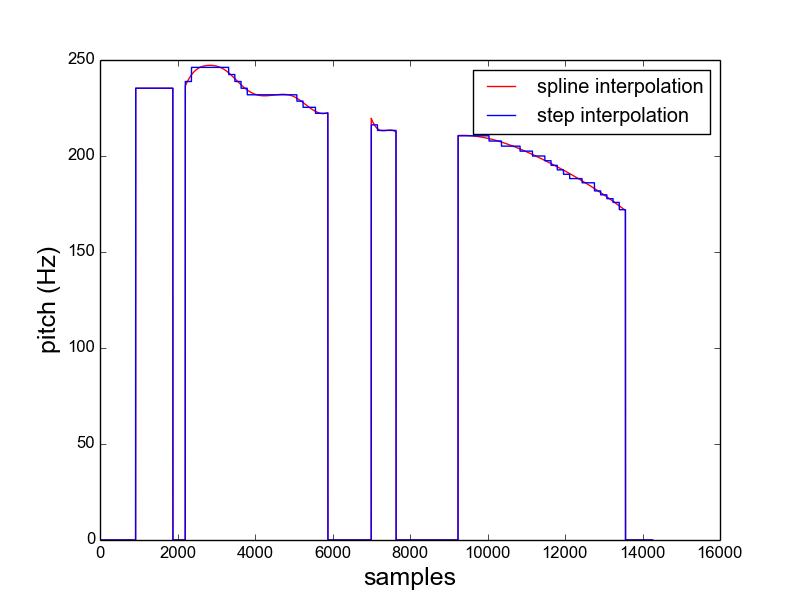
\includegraphics{interp.png}
\index{edges\_finder() (in module PitchObj)}

\begin{fulllineitems}
\phantomsection\label{pYAAPT:PitchObj.edges_finder}\pysiglinewithargsret{\code{PitchObj.}\bfcode{edges\_finder}}{\emph{values}}{}~\begin{quote}\begin{description}
\item[{Parameters}] \leavevmode
\textbf{values} (\emph{numpy array}) -- contains the low frequency energy for each frame.

\item[{Return type}] \leavevmode
list.

\end{description}\end{quote}

Returns the index of the samples where occur the transitions between unvoiced-voiced and voiced-unvoiced.

\end{fulllineitems}



\subsection{BandpassFilter Class}
\label{pYAAPT:bandpassfilter-class}
Creates a bandpass filter necessary for the YAAPT algorithm.

USAGE:
\index{BandpassFilter() (in module amfm\_decompy.pYAAPT)}

\begin{fulllineitems}
\phantomsection\label{pYAAPT:amfm_decompy.pYAAPT.BandpassFilter}\pysiglinewithargsret{\code{amfm\_decompy.pYAAPT.}\bfcode{BandpassFilter}}{\emph{fs}, \emph{parameters}}{}~\begin{quote}\begin{description}
\item[{Parameters}] \leavevmode\begin{itemize}
\item {} 
\textbf{fs} (\emph{float}) -- signal's fundamental frequency

\item {} 
\textbf{parameters} (\emph{dictionary}) -- contains the parameters options from the YAAPT algorithm.

\end{itemize}

\item[{Return type}] \leavevmode
bandpass filter object.

\end{description}\end{quote}

\end{fulllineitems}



\subsubsection{BANDPASS FILTER ATTRIBUTES:}
\label{pYAAPT:bandpass-filter-attributes}\index{b (in module BandpassFilter)}

\begin{fulllineitems}
\phantomsection\label{pYAAPT:BandpassFilter.b}\pysigline{\code{BandpassFilter.}\bfcode{b}}
Bandpass filter zeros coefficients. It is set during the object's initialization.

\end{fulllineitems}

\index{a (in module BandpassFilter)}

\begin{fulllineitems}
\phantomsection\label{pYAAPT:BandpassFilter.a}\pysigline{\code{BandpassFilter.}\bfcode{a}}
Bandpass filter poles coefficients. It is set during the object's initialization.

\end{fulllineitems}

\index{dec\_factor (in module BandpassFilter)}

\begin{fulllineitems}
\phantomsection\label{pYAAPT:BandpassFilter.dec_factor}\pysigline{\code{BandpassFilter.}\bfcode{dec\_factor}}
Decimation factor used for downsampling the data. It is set during the object's initialization.

\end{fulllineitems}


\begin{thebibliography}{ref1}
\bibitem[ref1]{ref1}{\phantomsection\label{pYAAPT:ref1} 
Stephen A. Zahorian, and Hongbing Hu, ``A spectral/temporal method for robust fundamental frequency tracking,'' J. Acosut. Soc. Am. 123(6), June 2008.
}
\end{thebibliography}



\renewcommand{\indexname}{Index}
\printindex
\end{document}
